\documentclass[22pt]{beamer}
\usepackage[orientation=portrait, size=custom, width=90.44, height=65,scale=1.2]{beamerposter} % 36in*2.5 = 90cm
\usepackage[absolute,overlay]{textpos}
\usepackage{bookmark} %pdflatex says to use this to avoid errors...
\usepackage{graphicx} %for including images
\graphicspath{{figs/}} %location of images
\usepackage{wrapfig} %wrap text around the images
\usepackage{listingsutf8}    %package for code environment; use this instead of verbatim to get automatic line break; use this instead of listings to get (•)
\usepackage{amsmath}
\usepackage{gensymb}
\usepackage[export]{adjustbox}
\usepackage[skins,theorems]{tcolorbox}
\usepackage{pgfplots}
\usepackage{tikz}
\usetikzlibrary{datavisualization}
\usetikzlibrary{datavisualization.formats.functions}
\usetikzlibrary{backgrounds}
\newcommand*\circled[1]{\tikz[baseline=(char.base)]{
            \node[shape=circle,draw,inner sep=2pt] (char) {#1};}}
\usepackage{array}
\usepackage{booktabs,adjustbox}
\usepackage{caption}
\captionsetup[figure]{font=scriptsize, labelfont=scriptsize}
\usepackage{ragged2e}
\usepackage{subfig}
\usepackage{xcolor}
\usepackage{scrextend}

\usepackage[english]{babel}
\usepackage{blindtext}

%\mode<presentation>
%this doesn't seem to make any difference; leave for now for trying out
\usetheme{Berlin}
\definecolor{MacBlue}{rgb}{0.10196,0.22353,0.53725}
\definecolor{MacMaroon} {rgb}{0.47843, 0, 0.23137}
\definecolor{MacMaroon2} {rgb}{0.47451, 0, 0}
\definecolor{MacGray}{rgb}{0.50196,0.49804,0.51765}
\definecolor{MacMaroon3}{rgb}{00.47,0.2,0.31}
\definecolor{MacGold}{rgb}{1, 0.75,0.35}
\usecolortheme[named=MacBlue]{structure}
\setbeamertemplate{caption}[numbered]
\setbeamertemplate{navigation symbols}{}
% \setbeamercolor{background canvas}{bg=MacGray}

\title{Hakaru Language: Standard Library Implementation and Language Validation Testing}
\subtitle{}  %probably want a better subtitle
  \author[Justin Staples, Mahmoud Khattab, Nevin Mahilal and Aryan Sohrabi]{Justin Staples, Mahmoud Khattab, Nevin Mahilal and Aryan Sohrabi, supervised by Dr.~Christopher Anand \& Dr.~Jacques Carette \vspace{0.3cm} \newline \small \{staplejw, khattm, mahilank, sohraa3, anandc, carette\}@mcmaster.ca}
  \institute[McMaster University]{\small{Department of Computing and Software, McMaster University}}
  \date{}

\newenvironment{variableblock}[3]{%
  \setbeamercolor{block body}{#2}
  \setbeamercolor{block title}{#3}
  \begin{block}{#1}}{\end{block}}

\begin{document}
%compile with pdflatex

%there is only one frame, because there is only one page; yeah, it's a poster
%textblock and block seem to work nicely to organize layout
\begin{frame}[fragile]

\begin{textblock}{2}(0.8,0.9)

\includegraphics[height=8.5cm]{mac.png}
\end{textblock}

\begin{textblock}{2}(12.9,0.6)
\includegraphics[height=11cm]{fireball.png} 
\end{textblock}

\begin{textblock}{8}(4,1)
\titlepage
\end{textblock}

\begin{textblock}{5}(0.25,3.5)

%%%%%%%%%%%%%%%%%%%%%%%%%%%%%%%%%%%%%%%%%%%%%%%%%%%%%%%%%%%%%%%%%%%%%%
% Introduction
%%%%%%%%%%%%%%%%%%%%%%%%%%%%%%%%%%%%%%%%%%%%%%%%%%%%%%%%%%%%%%%%%%%%%%

\begin{block}{\Large{Introduction}}
\justifying

\footnotesize{Hakaru is an experimental \textbf{probabilistic programming language}, which aims to simplify the implementation of statistical distributions. 

\begin{itemize}
    \item Niche application means that Hakaru is a small language with limited features.
    \item Running a hakaru program generates a stream of random numbers distributed according the statistical distribution modeled.
    \item Models can be compiled to C and Haskell for use in larger applications.
\end{itemize}

}

\bigskip
\footnotesize{{\tt \footnotesize{hk-maple}} is a provided inference algorithm that uses Maple to perform algebraic transformations on hakaru programs. In its default mode (Simplify), it returns an equivalent hakaru program with greater sampling efficiency. In applications requiring billions of samples (e.g. machine learning) this has the potential to save significant processing time!}

\end{block}

%%%%%%%%%%%%%%%%%%%%%%%%%%%%%%%%%%%%%%%%%%%%%%%%%%%%%%%%%%%%%%%%%%%%%%
% Motivation
%%%%%%%%%%%%%%%%%%%%%%%%%%%%%%%%%%%%%%%%%%%%%%%%%%%%%%%%%%%%%%%%%%%%%%

\begin{block}{\Large{Motivation}}
\justifying


\normalsize{\textbf{Objectives}}

\footnotesize{
\begin{itemize}
  \item Increase language accessibility: add new language features such as primivite mathematical functions (e.g. log, choose), new distributions, error handling, etc.
  \item Test language validity: use relationships between distributions to test the validity of program transformations like {\tt \footnotesize{hk-maple}}. 
\end{itemize}
}

\justifying

\normalsize{\textbf{Endeavours}}

\footnotesize{
\begin{itemize}
  \item Standard library development
  \item Syntax-highlighting-for-hakaru package for Sublime Text (Figures 2 and 3)
  \item Test case writing
  \item Filling in missing language features
\end{itemize}
        }

\end{block}


%%%%%%%%%%%%%%%%%%%%%%%%%%%%%%%%%%%%%%%%%%%%%%%%%%%%%%%%%%%%%%%%%%%%%%
% Key Concepts
%%%%%%%%%%%%%%%%%%%%%%%%%%%%%%%%%%%%%%%%%%%%%%%%%%%%%%%%%%%%%%%%%%%%%%

\begin{block}{\Large{Key Concepts}}
\justifying

\footnotesize{
\begin{itemize}
  \item[\textbf{$\star$}] \textit{Hakaru program $\Longleftrightarrow$ implementation of statistical distribution $\Longleftrightarrow$ probabalistic model $\Longleftrightarrow$ model.}
  \item[\textbf{$\star$}] \textit{Values pulled from a distribution are called measures. Measures $\Longleftrightarrow$ samples.}
  \item[\textbf{$\star$}] `{\textbf{$\sim$}}' vs `{\textbf{$<\sim$}}':
      \begin{itemize}
          \footnotesize
          \item[--] \footnotesize{$X \sim Normal(0, 1)$: random variable, $X$, is distributed according to a normal distribution (statistics literature).}
          \item[--] \footnotesize{{\tt \footnotesize{x $<\sim$ normal(0, 1)}}: pull a random sample from a normal distribution and bind it {\tt \footnotesize{x}} (Hakaru code).}
      \end{itemize}
  \item[\textbf{$\star$}] \textit{PDF: Probability Density Function (continuous distributions).}
  \item[\textbf{$\star$}] \textit{PMF: Probability Mass Function (discrete distributions).}
  \item[\textbf{$\star$}] \textit{UDR chart: Univariate Distribution Relationship chart.}
\end{itemize}
}
\end{block}


\begin{textblock}{5}(5.5,3.5)




%%%%%%%%%%%%%%%%%%%%%%%%%%%%%%%%%%%%%%%%%%%%%%%%%%%%%%%%%%%%%%%%%%%%%%
% Standard Library Development
%%%%%%%%%%%%%%%%%%%%%%%%%%%%%%%%%%%%%%%%%%%%%%%%%%%%%%%%%%%%%%%%%%%%%%

\begin{block}{\Large{Standard Library Development}}
\justifying

\footnotesize{Accessibility means the standard library implements commonly used statistical distributions. We have followed the UDR to implement distributions will the following guiding principles:


\footnotesize{

\bigskip
\begin{itemize}
  \item Whenever possible, implement distributions as transformations on pre-existing models.
  \item In the case of multiple possible implementations, take the shortest possible path from a primitive distribution on the UDR.
\end{itemize}
        }
}

\bigskip

\begin{figure}
\centering
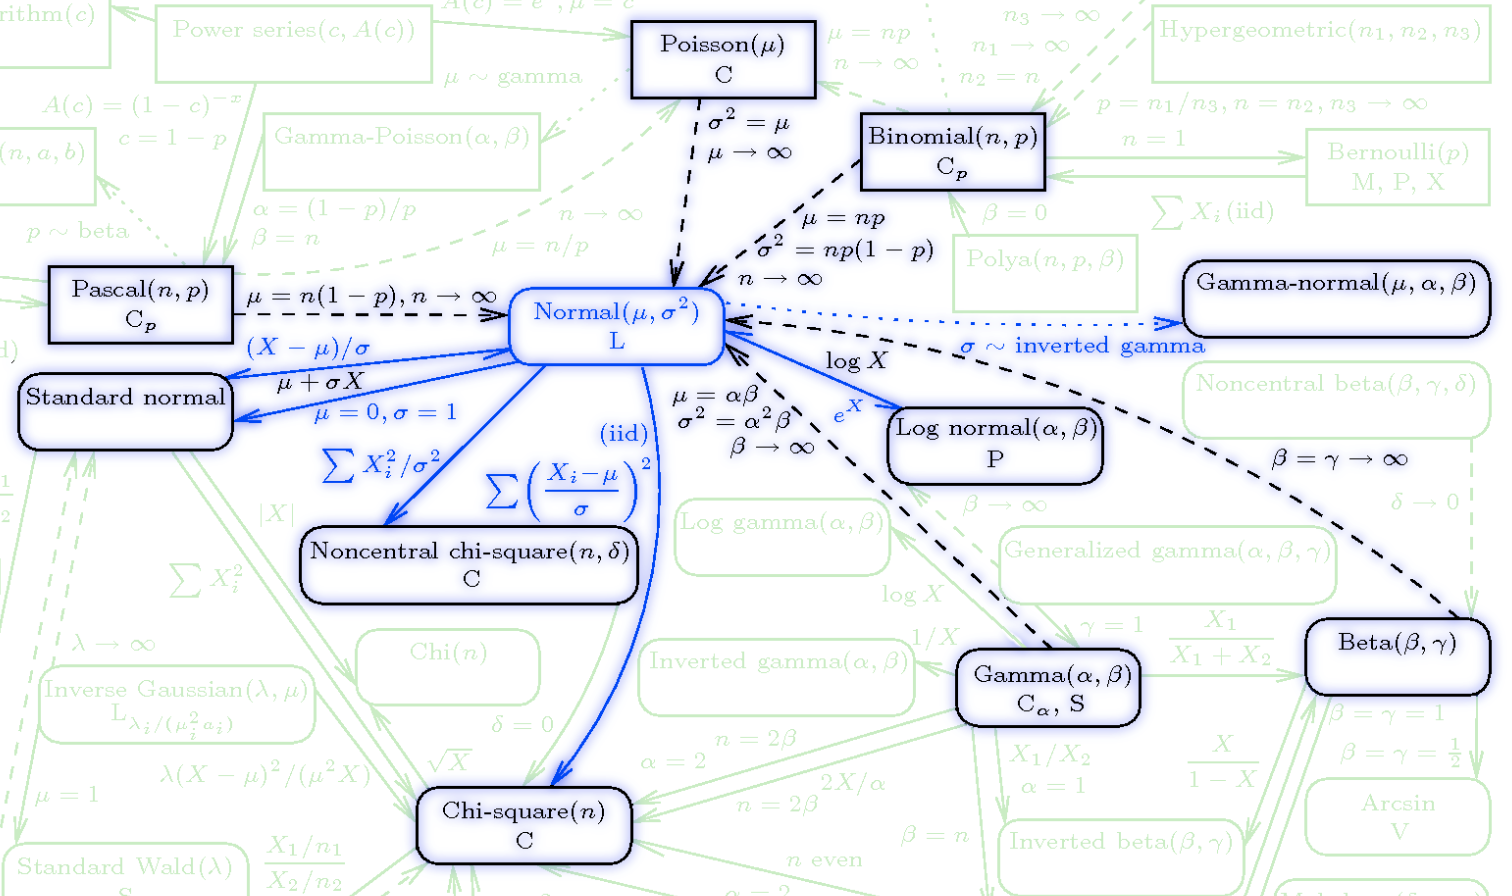
\includegraphics[height=12.5cm]{UDR.png}
\caption{\tiny{A snapshot of the UDR $^{[1]}$ shows how the normal distribution can be transformed into a multitude of other distributions.}}
\end{figure}

\footnotesize{Hakaru does not allow us to transform the model directly. Rather, we must apply transformations to samples pulled from the model using the bind {\tt \tiny{<$\sim$}} operator. Therefore, we are interested in implementing transformations of the form:}

\begin{equation*}
\begin{aligned}
& \tcboxmath[boxrule=2pt,colframe=MacMaroon]{R(p, q) \Rightarrow \textit{X} \sim A(p) \Rightarrow \textit{f(X)} \sim B(q)}
\end{aligned}
\end{equation*}

\bigskip

\footnotesize We can extend this definition to include transformations defined in terms of an aggregation of multiple independent samples. For example, the standard chi-square distribution is defined as the sum of the squares of \textit{n} normal random variables (see Figure 2). 

\bigskip
\begin{figure}
\centering
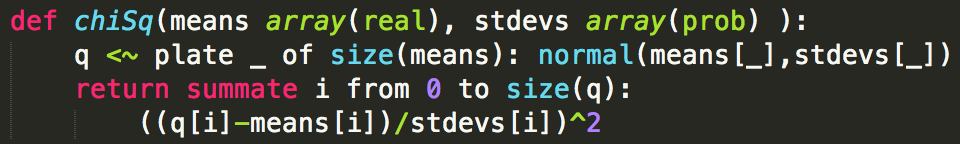
\includegraphics[height=3cm]{chi-square.png}
\caption{\tiny{Our implementation of the chi-square distribution.}}
\end{figure}

\bigskip
\footnotesize{Hakaru also lends itself well to Bayesian transformations, which take the following form. The gamma-poisson distribution can be described by such a transformation (see Figure 3).}

\begin{equation*}
\begin{aligned}
& \tcboxmath[boxrule=2pt,colframe=MacMaroon]{X \sim A(p) \Rightarrow Y \sim B(q, X) = C(p, q)}
\end{aligned}
\end{equation*}

~
~
~

\begin{figure}
\centering
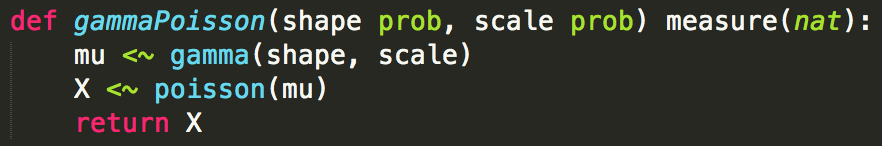
\includegraphics[height=3cm]{gamma-poisson.png}
\caption{\tiny{Our implementation of the gamma-poisson distribution.}}
\end{figure}

\end{block}



\end{textblock}

\end{textblock}


\begin{textblock}{5}(10.75,3.5)

\begin{variableblock}{}{}{}
\justifying

\footnotesize{In the case of unreachable distributions, we have resorted to defining models in terms of their PDF/PMF.}

\bigskip
\footnotesize{

By plotting a histogram of a sample polulation drawn from a distribution's model and comparing its shape to that of its PDF, we can have some confidence that the implementation is correct without proof.

}

\begin{figure}[!tbp]
  \centering
  \subfloat[]{ 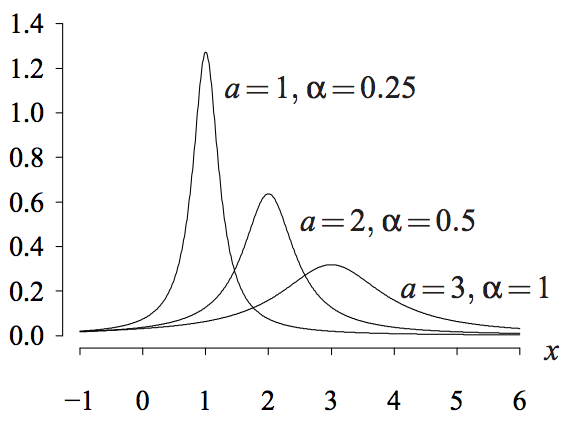
\includegraphics[width=0.38\textwidth]{cauchy.png}\label{fig:f1}}
  \subfloat[]{ 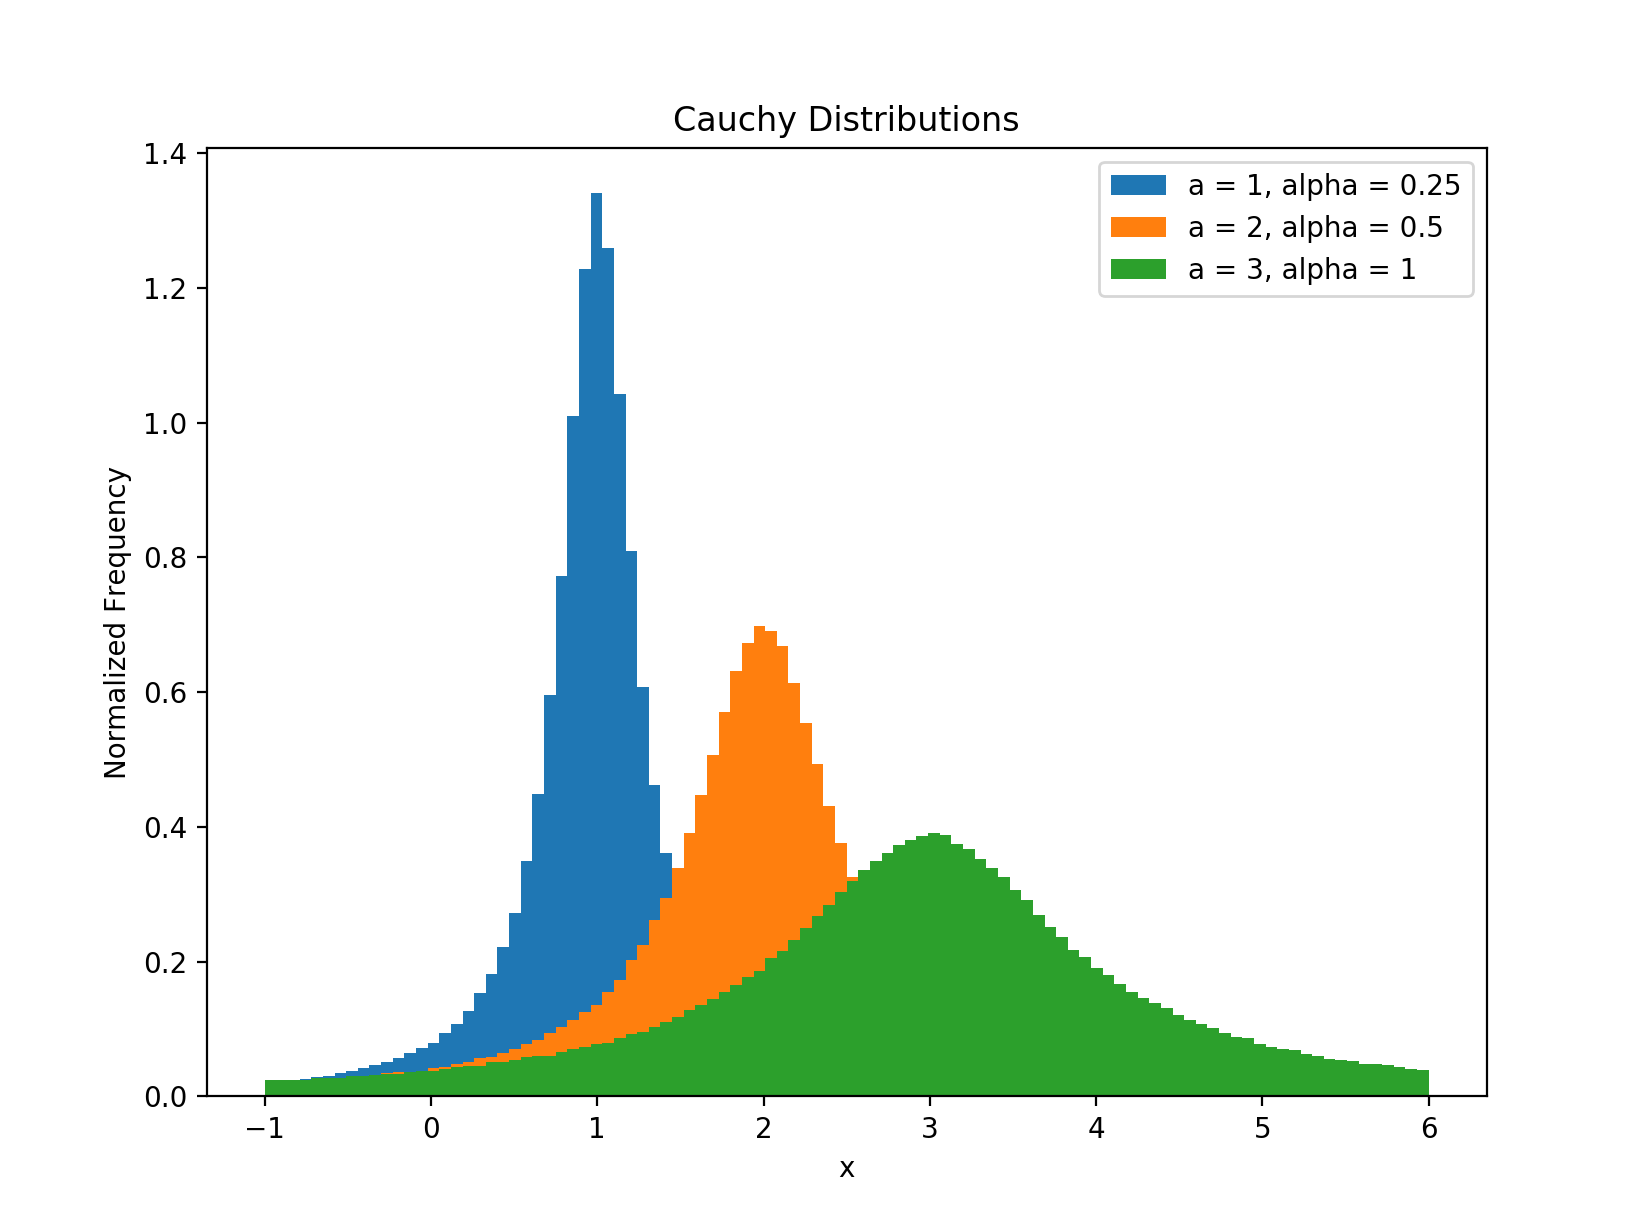
\includegraphics[width=0.38\textwidth]{cauchy_2.png}\label{fig:f2}}
  \caption{\tiny{A few plots of the Cauchy distribution are shown $^{[1]}$, along with a few histograms of data that have been sampled from a Hakaru program.}}
\end{figure}


\end{variableblock}

%%%%%%%%%%%%%%%%%%%%%%%%%%%%%%%%%%%%%%%%%%%%%%%%%%%%%%%%%%%%%%%%%%%%%%
% Testing Relationships Between Distributions
%%%%%%%%%%%%%%%%%%%%%%%%%%%%%%%%%%%%%%%%%%%%%%%%%%%%%%%%%%%%%%%%%%%%%%

\begin{block}{\Large{Testing Relationships Between Distributions}}
\justifying


\footnotesize{The validity of Hakaru can be tested by checking if it recognizes known relationships between distributions. More specifically:

\bigskip


\begin{addmargin}[4em]{4em}
\textit{Hypothesis: We hypothesize that by applying the appropriate transformations to implementations of A and B, we can create two Hakaru programs whose hk-maple outputs will be equivalent to each other. Test cases that prove our hypothesis true indicate the validity of the Hakaru language implementation. Test cases that prove our hypothesis false indicate an underlying bug in the language definition which is to be passed back to the language developers.}
\end{addmargin}

\bigskip
Given that test cases are written in Hakaru, we are limited to testing relationships of the form discussed. Our test cases focus on relationships involving a small set of distributions. Results are summarized below.

\bigskip
Tests that pass help prove that Hakaru is valid. Tests that fail either indicate a language bug, or are the consequence of an intended design choice. In all cases, these results give the language developers useful information for future work on the language.
}

\end{block}

%%%%%%%%%%%%%%%%%%%%%%%%%%%%%%%%%%%%%%%%%%%%%%%%%%%%%%%%%%%%%%%%%%%%%%
% Conclusions & Future Work
%%%%%%%%%%%%%%%%%%%%%%%%%%%%%%%%%%%%%%%%%%%%%%%%%%%%%%%%%%%%%%%%%%%%%%

\begin{block}{\Large{Conclusions \& Future Work}}

\footnotesize{This project was aimed at increasing language accessibility and testing the validity of Hakaru. A lot of ground was covered in both of these aspects in this project, but compared to other popular languages, Hakaru is still under development and has a lot of room for improvement. Here are just a few examples of where major development can still be done.

\begin{itemize}
    \item Languages features: Hakaru can be expanded further with new features like import statements and error/exception handling. 
    \item Standard library development: there are still many types of  distributions left to be implemented, such as multivariate distributions.
    \item Testing: There are a plethora of relationships between distributions that have yet to be investigated.  
\end{itemize}

}

\end{block}

%%%%%%%%%%%%%%%%%%%%%%%%%%%%%%%%%%%%%%%%%%%%%%%%%%%%%%%%%%%%%%%%%%%%%%
% References
%%%%%%%%%%%%%%%%%%%%%%%%%%%%%%%%%%%%%%%%%%%%%%%%%%%%%%%%%%%%%%%%%%%%%%

\begin{block}{\Large{References}}

\footnotesize{[1]~L. Leemis, "Univariate Distribution Relationship Chart", Math.wm.edu, 2018. [Online]. Available: http://www.math.wm.edu/~leemis/chart/UDR/UDR.html. 

[2]~P. Narayanan, J. Carette, W. Romano, C. Shan and R. Zinkov, “Probabilistic Inference by Program Transformation in Hakaru (System Defootnoteion)”, Functional and Logic Programming, pp. 62-79, 2016.}


\end{block}


% \begin{block}{References}
% \setbeamertemplate{bibliography item}{\insertbiblabel}
% \bibliographystyle{ieeetr}
% {\size
% \bibliography{../bib}}
% \end{block}

\end{textblock}
\end{frame}
\end{document}
